\section{Surfaces and their Classification}
\label{sec:surf}

We will finally be able to give a proper topological definition for
surfaces, and soon we will be able to state the theorem.

\subsection{Surfaces and Orientability}
\label{sec:surf:surfaces}

We begin by recalling the metric topology from example
\ref{exmp:metric}. With this topology in mind for the metric space
$\mathbb{R}^2$ under the Euclidean metric, we have the following
definition

\begin{defn}
  We say that $S$ is a \emph{surface} if it is a Hausdorff space for
  which every point has a neighbourhood that is homeomorphic to the
  open unit ball $\{\mathbf{x} \in \mathbb{R}^2 \mid \lvert \mathbf{x}
  \rvert < 1 \}$.
\end{defn}

We often implicitly like to deal with surfaces that are
\emph{connected} and \emph{compact} as discussed in section
\ref{sec:prelims:compact}.

We present the following examples.

\begin{exmp}
  The plane $\mathbb{R}^2$ is trivially a surface; each point is
  contained in $\mathbb{R}^2$, an open set that is homeomorphic to the
  unit ball $B_1(0)$ via $f:B_1(0) \rightarrow \mathbb{R}^2$, given by
  \[
    x \mapsto \frac{x}{x^2 - 1}.
  \]

  It is easy to see as a simple extension that any open subset of
  $\mathbb{R}^2$ is a surface.
\end{exmp}


We will see many more examples of surfaces in section
\ref{sec:surf:thm} but we will present one more example of a
surface. Here our example will be defined as a
\emph{quotient space}. The reader is advised to pay close attention to
this example as it shows how we can write a surface as a quotient
topology by identifying ``edges'' into the same equivalence class and
then considering it as a quotient space. This is analogous to
``cutting'' and pasting out different patches of a surface and is
better understood by example.

\begin{exmp}
  \label{exmp:mobius}
  Let $X$ be the subset of $\mathbb{R}^2$ that is equal to
  \[
    \{ (x,y) \in \mathbb{R}^2 \mid -10 \leq x \leq 10 ; -1 < y < 1 \}.
  \]
  Now, bearing in mind our discussion from section
  \ref{sec:prelims:quotient}, we \emph{identify} the points $(-10,-y)$
  and $(10,y)$ for $y \in (-1,1)$. In other words we define the
  quotient space $X^*$ to consist of points $(x,y)$ in their own
  equivalence class for $-10 < x < 10$ and $-1 < y < 1$ while the
  points $(-10,-y)$ and $(10,y)$ are each in the same equivalence
  class. We call the latter class of points ``identified'' points.

  This quotient topology $X^*$ is indeed a surface; we call this
  surface the M\"obius strip. Our action of identifying opposite
  points on the short edges is equivalent to ``gluing'' the short
  edge $a$ in reverse as pictured in Figure
  \ref{fig:mobius}. Conversely, the surface pictured in (b) can be
  ``cut'' along $a$ and laid out to form the quotient topology $X$
  that is pictured in (a). 
  
  To see that $X^*$ is indeed a surface, we consider any point
  $\mathbf{x}_0 \in X^*$. If $\mathbf{x}_0$ is not an identified point, it
  has a unique preimage $\mathbf{y}_0 \in X$ under the identification
  map $\pi$. Since $\mathbf{y}_0$ lies in the interior of the rectangle
  $X$, we can find a ball $B$ that is also contained in the interior
  of $X$. Clearly $B' = \pi(B)$ is open in $X^*$ and contains
  $\mathbf{x}_0$. It is easy to show that a restriction of $\pi$ to $B$
  is a homeomorphism and it follows from this that $B'$ is
  homeomorphic to the unit ball.

  If however $\mathbf{x}_0 = \{ (10,y_0) (-10,-y_0) \}$ is an
  identified point, it's preimage under $\pi$ would be two points on
  the short  edge of $X$, say $\mathbf{x_1}$ and $\mathbf{x_2}$ which
  are equidistant from the nearest long boundary of  X. Suppose $B_1$
  and $B_2$ are balls centered around $\mathbf{x_1}$ and
  $\mathbf{x_2}$ of radius $R$ that do not touch the long edge of
  $X$. Set $B = (X \cap B_1) \cup (X \cap B_2)$ and $B' =
  \pi(B)$. Then, $B'$ is a neighbourhood of $\mathbf{x}$ that is
  contained in $X^*$. This is indeed homeomorphic to the unit ball in
  $\mathbb{R}^2$. To see this consider $\phi: B_1(\mathbf{0})
  \rightarrow B'$ given by 
  \[
    \phi((x,y)) =
    \begin{cases}
      (Rx + 10, Ry + y_0), & \text{if $x < 0$} \\
      \{(10, Ry + y_0),(-10, Ry - y_0)\}, & \text{if $x = 0$} \\
      (Rx - 10, Ry - y_0), & \text{if $x > 0$}.
    \end{cases}
  \]

  This is indeed a homeomorphism, thus $X^*$ is
  a surface\footnote{Our classification theorem will only talk about
    surfaces without a boundary. Thus the theorem will not classify
    the M\"obius strip, which has a boundary.}.
  % proceed by finding for each element $\mathbf{x}$ of $X^*$ an open
  % neighbourhood characterised by a radius $r > 0$. Then we will show
  % that our choice is homeomorphic to the unit ball on $\mathbb{R}^2$
  % and finally we will show that given any two points the
  % neighbourhoods can be chosen such that they don't intersect
  % (Hausdorff condition).

  % Assume that $\mathbf{x}$ isn't identified. This point is mapped by
  % the projection map $\pi$ from a unique point in the interior of the
  % rectangle $X \subseteq \mathbb{R}^2$. Working in this open rectangle
  % as a metric space, we can find open balls given by radius $r >0$
  % that is entirely contained in the interior of the rectangle. Now
  % map this ball back to $X^*$ via $\pi$ and denote this set by
  % $B_r(\mathbf{x}) \subseteq X^*$.
  
  % Since the ball was contained in the interior of the rectangle, no
  % point in them is identified, so the projection's restriction to the
  % open ball in $X$ is invertible. It follows that $\pi^{-1}
  % (B_r(\mathbf{x}))$ is exactly the ball that we started with and is
  % open in $X$, so by definition of the quotient space
  % $(B_r(\mathbf{x}))$ is an open neighbourhood of $\mathbf{x}$.

  % In the case that $\mathbf{x}$ is an identified point, its pull-back
  % is the pair of points $\pm(10, y)$ on the border of $X$. Given $0 <
  % r < \operatorname{min} \{ 1-y, -1-y \}$, let $U_r(\mathbf{x})$ be
  % the intersection of the two open balls of radius $r$ about $\pm(10,
  % y)$ with $X$. We define the image of $U_r(\mathbf{x})$ under the
  % projection $\pi$ to be $B_r(\mathbf{x})$. Now it is easy to see that
  % the preimage of $B_r(\mathbf{x})$ under $\pi$ is $U_r(\mathbf{x})$,
  % which is open in the subspace $X$. It follows that $B_r(\mathbf{x})$
  % suffices as a neighbourhood for $\mathbf{x}$.

  % It is important to note however that we haven't defined quotient
  % subspace $X^*$ and our notation $B_r(\mathbf{x})$ similar to that of
  % open balls in metric spaces is only notional and will help with
  % intuition later on.

  \begin{figure}[htbp]
  \centering
  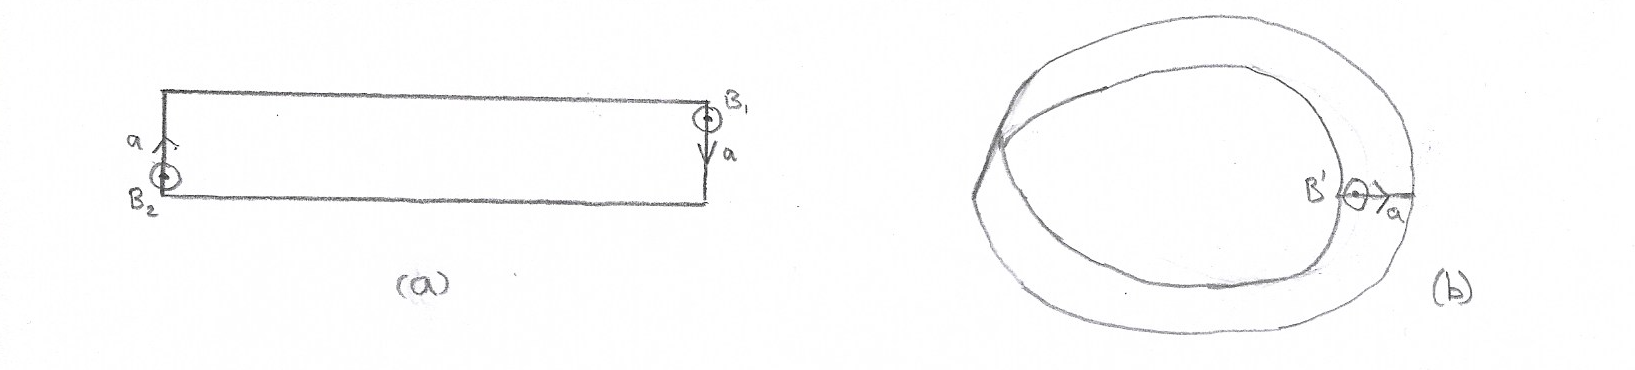
\includegraphics[width=13.5cm]{mobius.png}
  \caption{The M\"obius strip as a quotient topology formed by
    identifying opposite edges of a rectangle.} 
  \label{fig:mobius}
\end{figure}
\end{exmp}

This example is notable because it shows that surfaces can be
equivalently written as themselves that are  ``cut-up'' albeit
remembering which edges of the cut-up surface are ``to be
identified''. This information of which edges are to be identified is
conveyed by writing the cut-up surface as a quotient topology. We will
use this technique extensively in the next section (and throughout the
rest of this document) as we show that an arbitrary surface can be
``cut-up'' into triangles that are ``to be identified''.

\subsection{Triangulation}
\label{sec:surf:triangulation}

We define what it means to triangulate a surface.

\begin{defn}
  Given a surface $S$, we say that the collection of closed sets $\{
  T_1,  T_2, \dots T_n \}$ \emph{triangulates} $S$ if it covers $S$
  and for each $i = 1,2, \dots, n$ there exists homeomorphisms $\phi
  : T_i' \rightarrow T_i$ where each $T_i'$ is a triangle in
  $\mathbb{R}^2$ under the metric topology (described in example
  \ref{exmp:metric}). We say that the \emph{edges} of $T_i$ are images
  of the edges of $T_i'$ for each $i$; similarly the \emph{vertices}
  of $T_i$ are the images of the vertices of $T_i'$.
\end{defn}

We take it as a fact that any compact surface can be triangulated. We
understand that this is the case from the Jordan Curve theorem but
showing this goes beyond the scope of this project. To see a proper
discussion of how arbitrary compact surfaces can be triangulated,
refer to \cite{thom}.

Given that an arbitrary surface $S$ can be triangulated, we make
``cuts'' along the edges of the triangles and notice that each
triangle can be ``pasted'' onto the plane $\mathbb{R}^2$. Since
translations are homeomorphisms as well, we can translate the
triangles appropriately and have all triangles from the triangulation
``pasted'' on the plane in a manner by which they do not intersect
each other.

More formally, we begin by inductively relabeling our
triangulation. Suppose we have $n$ ``triangles'' that cover $S$; then
we proceed to label them inductively starting by labeling any
triangle $T_1$. Then, for each $1 \leq i \leq n-1$, choose a $T_{i+1}$
that has an edge $e_i$ in common with one of the preceding
triangles $T_1, T_2, \dots, T_i$. Such a triangle must always exist by
our implicit assumption of the connectedness of $S$. Numbering  our
triangle in this manner, we have defined the edges $e_i$ for $2 \leq i
\leq n$. 

For each triangle $T_i$ we must by definition have a homeomorphism
$\psi_i: T_i' \rightarrow T_i$, where $T_i'$ is a triangle in
$\mathbb{R}^2$. Translating the triangles $T_i'$ to $T_i''$ such that
they are pairwise disjoint, it is clear that there exists
homeomorphisms $\phi_i: T_i'' \rightarrow T_i$. Finally, given $T'' =
\cup_{i=1}^n T_i''$ and $\phi : T'' \rightarrow S$ defined via $\phi
\restriction T_i = \phi_i$ it is easy to see that $\phi : T''
\rightarrow S$ is a homeomorphism. 

For now, we assume that our surface $S$ doesn't have a
boundary and as a result each triangle edge has a corresponding edge %% what is a boundary?
on some other triangle that it is identified with.

Here we have explained how an arbitrary compact surface can be written
as finitely many triangles pasted on the plane \emph{under the
  quotient topology} that identifies pairs of edges. It is important
to note that we must include the added information of which edges are
identified with each other when we represent this quotient space, and
also include in what direction they are to be glued on. In 
particular we will represent this quotient space as the triangle that
forms it with each edge labeled and an it's identification
``direction''. We have already seen in Figure \ref{fig:mobius} how we
may imagine this space, where each edge is labeled with an arrow
indicating which direction it is to be identified with it's
corresponding edge.

We will show that the triangles of this quotient space can be
``glued'' onto one another so that we end up with a quotient space on
a geometric shape that is topologically equivalent to a disc. We do
this as follows.

It is clear that each $T_i$ is homeomorphic to a closed
disc. Furthermore, we have that the edges of $T_i$ are homeomorphic to
``closed'' boundaries on the disc, i.e.\ a set $A$ on the boundary of 
the disc that is homeomorphic to $[0,1]$. Now identifying two such
closed boundaries $A_1$ and $A_2$ we can identify them via the
homeomorphism between them and the resulting quotient space is
homeomorphic to a disc !(discuss). Hence, starting by deforming $T_1$
into a disc $D_1$, we proceed by gluing $T_i$ onto the edge $e_i$ of
the disc $D_{i-1}$ and continuously deform the resulting quotient
space into a disc $D_i$ for $2 \leq i \leq n$. Composing each gluing
and deformation, we have a surjective function $\pi$ from our quotient
space of triangles $T_1, T_2, \dots T_n$ to the disc $D_n$. Lemma
\ref{lem:prelims:compose} confirms that $\pi$ induces the quotient
topology on $D_n$ that is consistent with gluing each triangle and
deforming it into a disc one by one. As a result the boundary of the
disc entirely consists of the remaining pairs of edges i.e.\ not $e_2,
e_3, \dots, e_n$. Figure \ref{fig:square-pyramid} shows this process
being done for a square pyramid.

\begin{figure}[htbp]
  \centering
  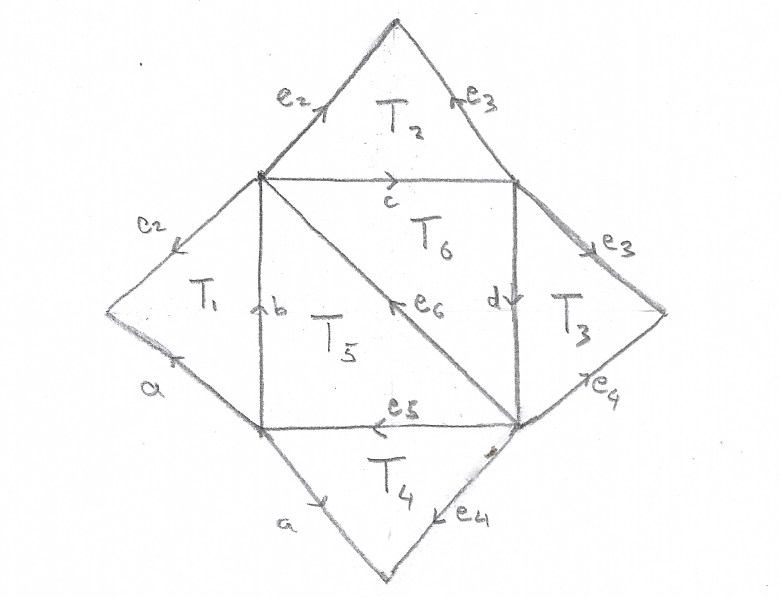
\includegraphics[width=8cm]{pyramid.png}
  \caption{Triangulating a square pyramid and forming its ``polygon''.}
  \label{fig:square-pyramid}
\end{figure}

This is significant since we formed a ``polygon'' that is homeomorphic
to an arbitrary compact and connected surface. Furthermore, if we
label the edges of the polygon, we can form a ``word'' that represents
the surface by going around the polygon counter-clockwise and picking
up the labels, with an inverse sign depending on the direction we
encounter them, and collating them. 

\subsection{Stating the Classification Theorem}
\label{sec:surf:thm}

Now that we know that a compact, connected surface $S$ can be written
as a polygon's quotient space all we seemingly need to do is classify
such polygons. Here we state the main theorem

\begin{thm}
  \label{thm:main}
  Any compact, connected surface without a boundary is either
  homeomorphic to a sphere, or to a connected sum of tori, or to a
  connected sum of projective planes. 
\end{thm}

We will now describe these ``prototype'' surfaces and show how they
can be written as polygons (and thus ``words'') as we did in section
\ref{sec:surf:triangulation}. Finally, we will show how an arbitrary
$D_n$ as formed in \ref{sec:surf:triangulation} can be reduced into
one of our ``prototype polygons''.


\subsubsection{The Sphere, Torus and Projective Plane}
\label{sec:surf:thm:stp}

Here we describe the prototype surfaces that are orientable, namely
the sphere and n-tori. The sphere is the simplest orientable surface
that we encounter. We can ``cut'' a slit along a diameter, pull the
sphere open and flatten it to form a bigon under the quotient topology
as demonstrated in figure \ref{fig:sphere-bigon}.

\begin{figure}[htbp]
  \centering
  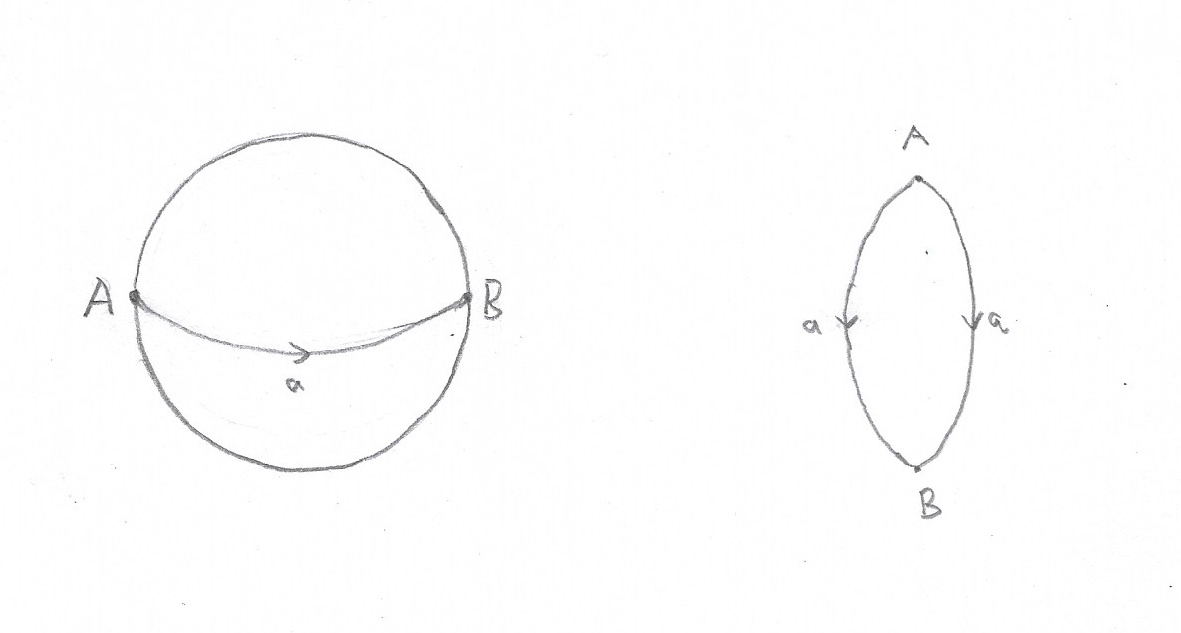
\includegraphics[width=14cm]{sphere.png}
  \caption{Representing the sphere as a bigon.}
  \label{fig:sphere-bigon}
\end{figure}

This polygon's quotient topology can be written, starting from the top
vertex and going counter-clockwise, as  the ``word''
$aa^{-1}$. Another simple surface that can be represented as a bigon,
albeit non-orientable is the projective plane; it is represented by
the quotient topology in figure
\ref{fig:projective-plane-bigon}. The corresponding word for this surface
is clearly of the form $aa$.

\begin{figure}[htbp]
  \centering
  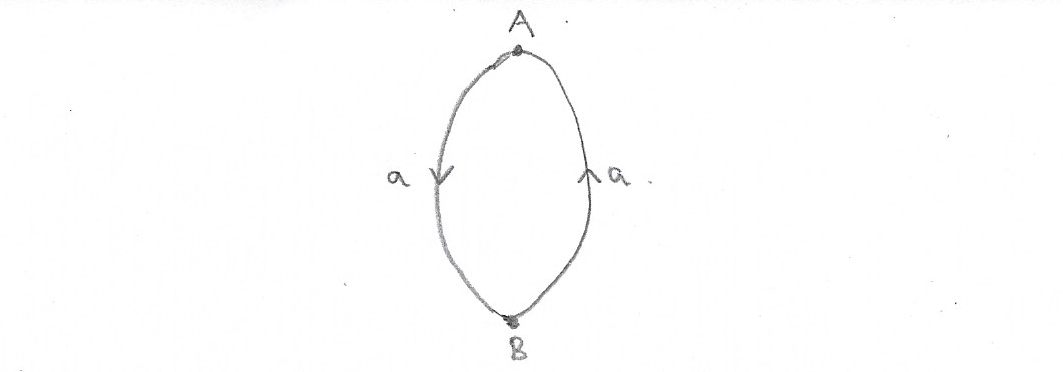
\includegraphics[width=13.5cm]{projective.png}
  \caption{The projective plane.}
  \label{fig:projective-plane-bigon}
\end{figure}

The last basic surface that we present in this section is the torus,
which is a simple tube whose edges are glued onto each other
(identified). This can be represented as a quadrilateral as in figure
\ref{fig:torus-rectangle}. The corresponding ``word'' takes the form
$aba^{-1}b^{-1}$ 

\begin{figure}[htbp]
  \centering
  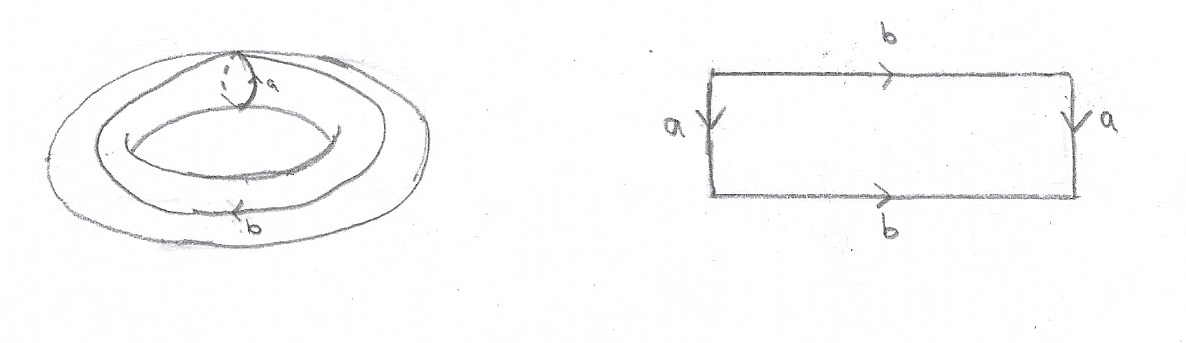
\includegraphics[width=8cm]{torus.png}
  \caption{Identifying edges of a rectangle to form a torus.}
  \label{fig:torus-rectangle}
\end{figure}

\subsubsection{Connected Sums}
\label{sec:surf:thm:cs}

For two disjoint surfaces, their connected sum is formed by deleting
circular holes in the surface and gluing the boundaries of the holes
to each other. More precisely we can do this to surfaces $S_1$ and
$S_2$ by taking two neighbourhoods $U_1 \subseteq S_1$ and $U_2
\subseteq S_2$ that are homeomorphic to the open unit disc via
$\phi_1$ and $\phi_2$. If $B_1$ and $B_2$ are open balls of radius
$\frac{1}{2}$ in the respective images of $\phi_1$ and $\phi_2$, we
form the connected sum $S$ by deleting the preimages of the interiors
of $C_1$ and $C_2$, i.e.\ we have $S_1' := S_1 \setminus
\phi_1^{-1}(B_1)$ and $S_2' := S_2 \setminus
\phi_2^{-1}(B_2)$. Finally we glue the boundaries of the deleted
balls, that is, we identify points in $\phi_1^{-1} (\partial B_1)
\subseteq S_1'$ with those in $\phi_2^{-1} (\partial B_2) \subseteq
S_2'$ to form our connected sum $S$ of $S_1$ and $S_2$. We know that
this can indeed be done since both are homeomorphic to circles in
$\mathbb{R}^2$.

First, we will study how connected sums of tori are formed. We already
know that tori can be written as quadrilaterals with opposite edges
identified; thus we can write  two tori $T_1$ and $T_2$ as
$a_1b_1a_1^{-1}b_1^{-1}$ and $a_2b_2a_2^{-1}b_2^{-1}$
respectively. Now cut out closed loops $c_1$ and $c_2$ in $T_1$ and
$T_2$ that run through the vertices  $a_1b_1^{-1}$ and $a_2b_2^{-1}$
respectively, as in figure \ref{fig:2-tori}. Now we identify the $c_1$
with $c_2$ to form the 2-torus represented by the polygon
$a_1b_1a_1^{-1}b_1^{-1}a_2b_2a_2^{-1}b_2^{-1}$.

\begin{figure}[htbp]
  \centering
  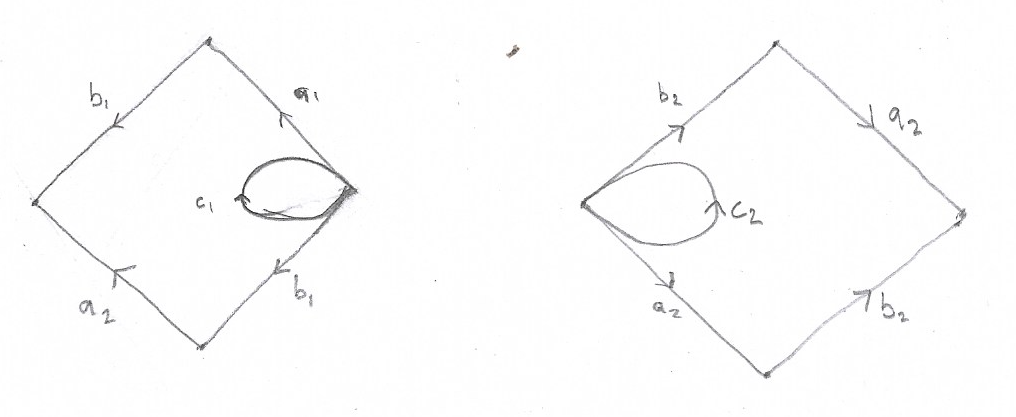
\includegraphics[width=12cm]{2torus.png}
  \caption{The 2-torus}
  \label{fig:2-tori}
\end{figure}

Cutting a loop that passes through the vertex between $a_1$ and
$b_2^{-1}$ we can connect another torus that we write as
$a_3b_3a_3^{-1}b_3^{-1}$ as we did above to form a $3-torus$ of the
form
$a_1b_1a_1^{-1}b_1^{-1}a_2b_2a_2^{-1}b_2^{-1}a_3b_3a_3^{-1}b_3^{-1}$. This
can be repeated $n$ times and thus an n-torus can be written as the
word $a_1b_1a_1^{-1}b_1^{-1}a_2b_2a_2^{-1}b_2^{-1} \dots
a_nb_na_n^{-1}b_n^{-1}$.

This process can be done to the projective plane as well by cutting
holes and gluing as in figure \ref{fig:2-projective-plane}. The word
we arrive at after one iteration is $a_1a_1a_2a_2$, but it is easy to
see that the connected sum of $n$ projective planes can be written as
the word $a_1a_1a_2a_2 \dots a_na_n$.

\begin{figure}[htbp]
  \centering
  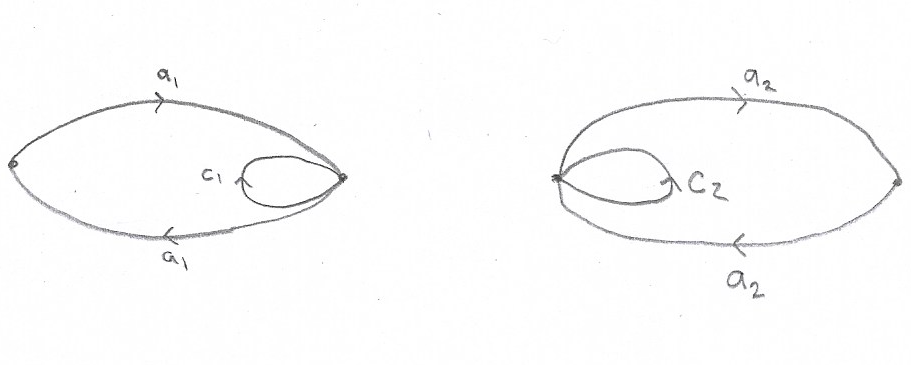
\includegraphics[width=12cm]{2projective.png}
  \caption{Connected sums of projective planes}
  \label{fig:2-projective-plane}
\end{figure}

With this we have introduced all of our prototype surfaces and  we
will proceed to present a lemma that will prove useful in proving the
classification theorem. 

\begin{lem}
  \label{lem:connected}
  The connected sum of a torus and a projective plane is homeomorphic
  to the connected sum of three projective planes. 
\end{lem}

Before we prove this lemma, it will be helpful to take a look at the
following example.

\begin{exmp}
  \label{exmp:klein} A Klein bottle is a non-orientable surface formed by identifying
  edges of a rectangle as in figure \ref{fig:klein}. We will see that
  this surface is equivalent to the connected sum of two projective
  planes.
  \begin{figure}[htbp]
    \centering
    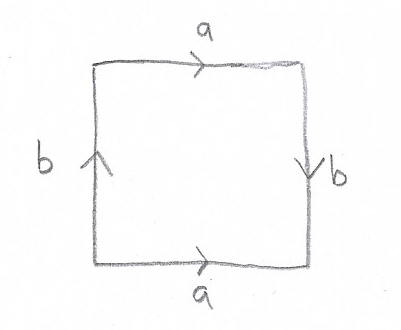
\includegraphics[width=8cm]{klein.png}
    \caption{The Klein Bottle}
    \label{fig:klein}
  \end{figure}
  Cutting out a disc $D_1$ from a projective plane $S_1$, we
  observe that the surface $S_1 \setminus D_1$ is a M\"obius strip as
  can be seen in figure \ref{fig:mob-proj}.
  \begin{figure}[htbp]
    \centering
    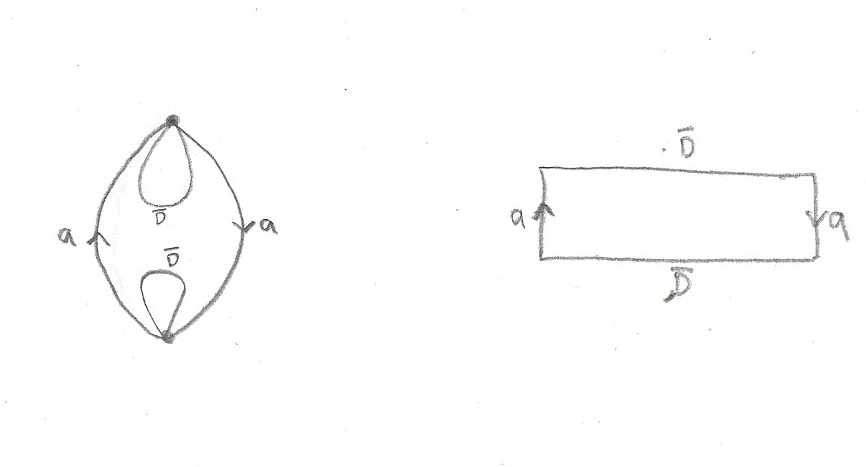
\includegraphics[width=13.5cm]{mobdisk.png}
    \caption{The M\"obius strip is a projective plane with a disc deleted}
    \label{fig:mob-proj}
  \end{figure}
  Thus, the connected sum of two projective planes $S_1$ and $S_2$
  must be two M\"obius strips glued onto one another at the
  boundary. From  figure \ref{fig:klein}, it is easy to see that this
  is indeed a Klein bottle.
\end{exmp}

\begin{proof}
  By example \ref{exmp:klein}, our problem is reduced to showing that
  the connected sum of the projective plane and Klein bottle is
  homeomorphic to the connected sum of the projective plane and
  torus. The canonical quotient spaces representation for the Klein
  bottle and torus with discs deleted are shown in figure
  \ref{fig:tor-klein}.
  \begin{figure}[htbp]
    \centering
    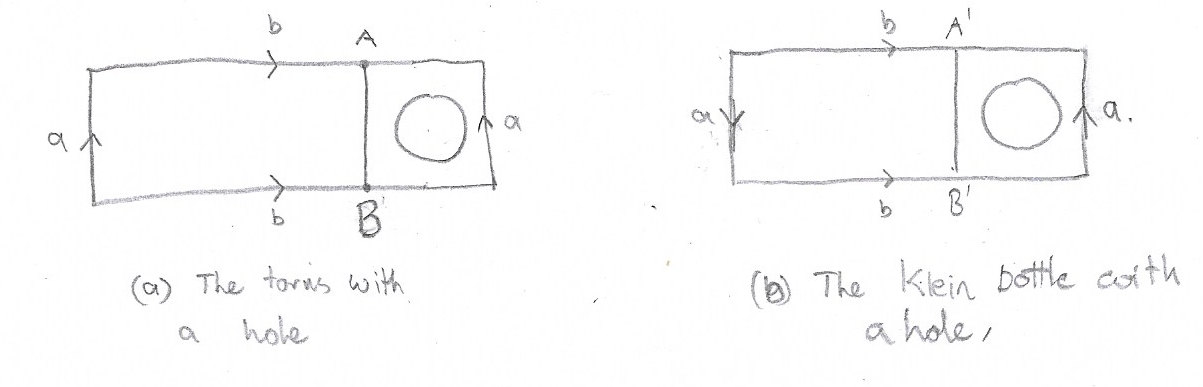
\includegraphics[width=13.5cm]{torklein.png}
    \caption{The torus and Klein bottle}
    \label{fig:tor-klein}
  \end{figure}

  We make cuts along $AB$ and $A'B'$, to form the edge $a'$. Gluing
  the hole in these cutoffs onto a hole in a segment of a surface is
  represented in figure \ref{fig:glue-S}. We have our surface with two
  holes to which the remainder of the Klein bottle or torus must be
  identified.

  \begin{figure}[htbp]
    \centering
    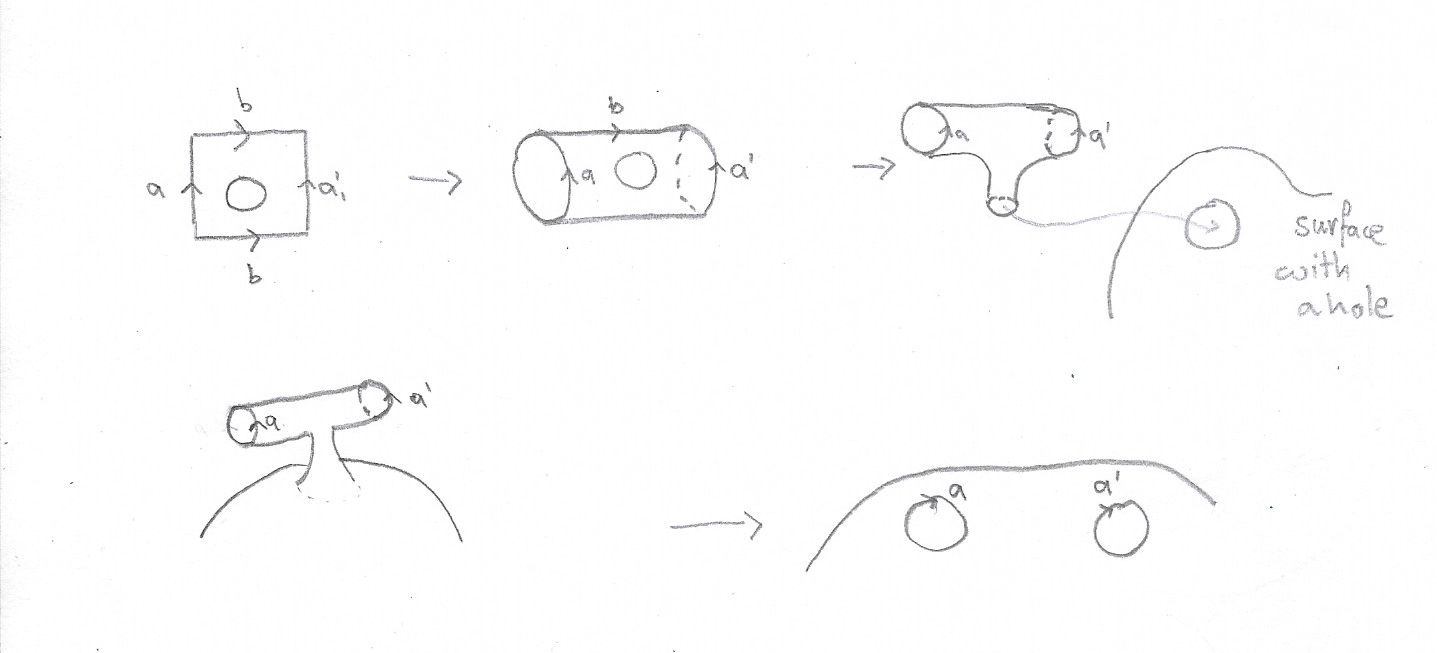
\includegraphics[width=13.5cm]{glues.png}
    \caption{The first step of gluing the torus and Klein bottle onto
      a surface segment}
    \label{fig:glue-S}
  \end{figure}

  In our second stage of gluing we want to re-attach the segment we cut
  away in figure \ref{fig:tor-klein}. Here we will suppose that the
  surface we are gluing to is a M\"obius strip. The completion of the
  second stage in both the case of the torus and the Klein bottle is
  seen in figure \ref{fig:glue-mob}, working in the M\"obius strip as a
  quotient topology that is cut apart at $m$.
  
  \begin{figure}[htbp]
    \centering
    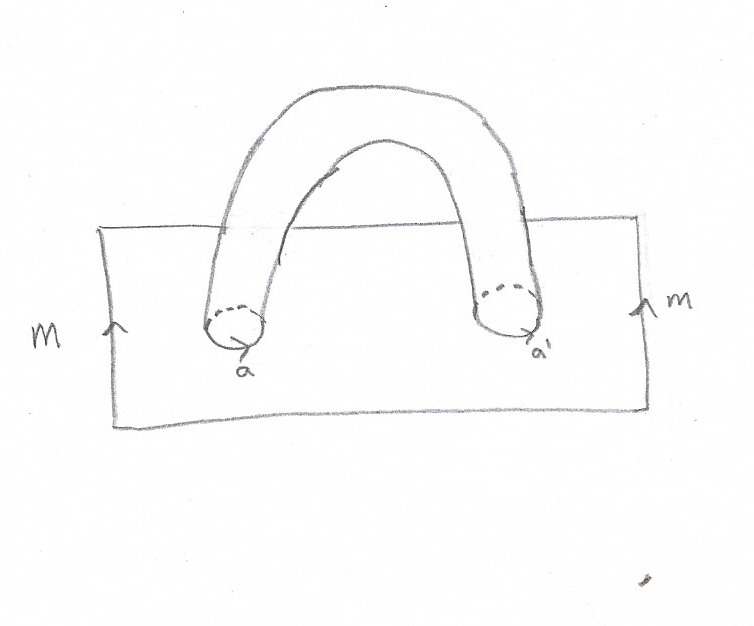
\includegraphics[width=8cm]{gluemob.png}
    \caption{The connected sums of the torus and the Klein bottle with
      the M\"obius strip}
    \label{fig:glue-mob}
  \end{figure}
  Since the M\"obius strip is simply a projective plane with a disc cut
  out as seen in example \ref{exmp:klein}, we just could have
  identified the boundary of a disc with the boundary of the M\"obius
  strip and have our result.
\end{proof}

In summary the canonical forms given in theorem \ref{thm:main} can be
written as follows. 

\begin{itemize}
\item The sphere, written as $aa^{-1}$.
\item The connected sum of $n$ tori,  written as
  $a_1b_1a_1^{-1}b_1^{-1}a_2b_2a_2^{-1}b_2^{-1} \dots
  a_nb_na_n^{-1}b_n^{-1}$.
\item The connected sum of $n$ projective planes, written as
  $a_1a_1a_2a_2 \dots a_na_n$.
\end{itemize}

 \begin{proof}[Proof of the Classification Theorem]
   This now simply boils down to showing that the polygon $D_n$ that
   we constructed from an arbitrary surface in section
   \ref{sec:surf:triangulation} is homeomorphic to one of the three
   above forms. We do this by manipulating $D_n$ in a systematic way
   to arrive at one of these forms.

   First, we will classify the pairs of edges of $D_n$. We say that
   pairs that occur in opposite directions are \emph{pairs of the
     first kind}; an edge with the label $a$ will occur as a pair of
   the first kind in $D_n$ if $D_n$'s word has the exponents of the
   two occurrences of the label $a$ not equal. In other words, $a$ and
   $a^{-1}$ both appear in the word representing $D_n$. For example a
   sphere is nothing but a pair of the first kind. On the other hand
   we call \emph{pairs of the second kind} those pairs who both have
   the same exponents. For example a projective plane is simply a
   single pair of the second kind.

   We can eliminate adjacent pairs of the first kind in any polygon
   with more than two pairs by simply identifying the pair as seen in
   \ref{fig:first-adjacent}. Thus $D_n$ can be reduced to a polygon
   with no adjacent pairs of the second kind or a bigon, which we know
   is equivalent to either a sphere or a projective plane. In the
   latter case we are done so assume that $D_n$ is reduced to $P$, a
   polygon with no adjacent edges of the first kind. Figure
   \ref{fig:square-pyramid} is found to be homeomorphic to the sphere
   by this step.

   \begin{figure}[htbp]
     \centering
     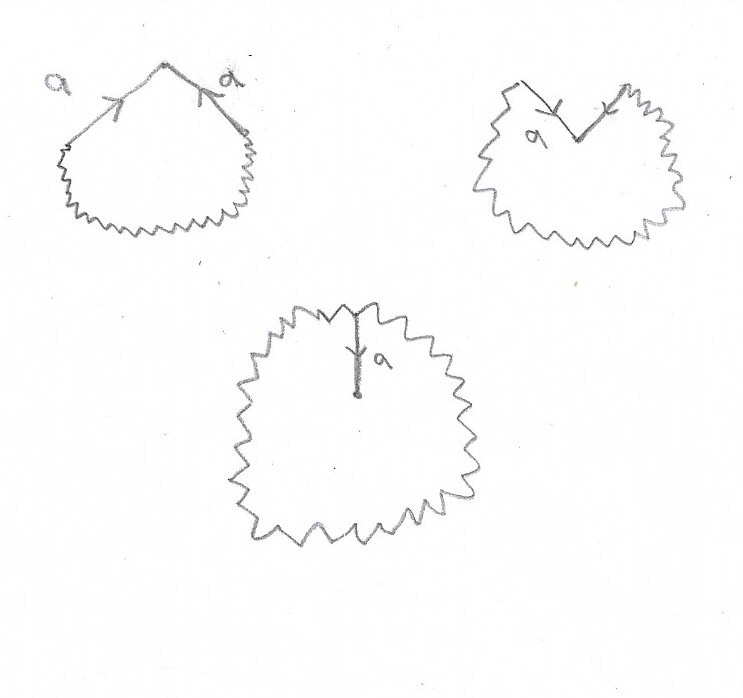
\includegraphics[width=8cm]{first.png}
     \caption{Eliminating adjacent pairs of the first kind.}
     \label{fig:first-adjacent}
   \end{figure}

    Just as edges were formed by cutting and are to be reidentified, so
    are vertices; however, unlike edges, vertices need not be identified
    in pairs. Rather, an equivalence class of vertices may have any
    finite number of vertices along the polygon $P$. 
    
    We claim that all but one equivalence class of vertices can be
    eliminated via homeomorphic actions on the polygon $P$. Suppose
    there are at least two equivalence classes of vertices. In this
    case, we will show that an arbitrary equivalence class $A$ can be
    eliminated. This will clearly lead to our claim being verified
    since we have finitely many equivalence classes of vertices.

    $A$ must have a vertex that is adjacent to a vertex of a different
    equivalence class, say $B$. Since we have eliminated adjacent
    pairs of edges the first kind, an equivalence class of vertices
    such as $A$ must have more than one vertex, therefore without loss
    of generality we can represent our situation as in figure
    \ref{fig:vertex-eliminate} (a). With this figure in mind, 
    cut the polygon along $c$ and identify the pair of edges $a$, as
    pictured in part (b) of the figure. We now have one fewer vertex
    of the equivalence class $A$ and one more of the equivalence class
    $B$. Now, apply the first step again (eliminate adjacent pairs of
    the first kind). Either this will eliminate the class $A$ if a
    single vertex remains, or we will have the conditions required to
    repeat this procedure till finally $A$ is eliminated.
    
    \begin{figure}[htbp]
     \centering
     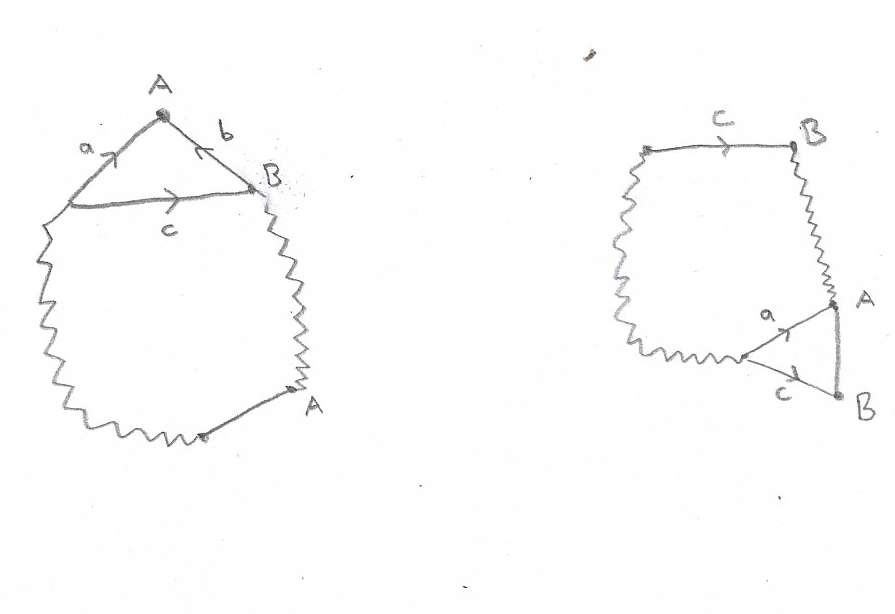
\includegraphics[width=10cm]{vertex.png}
     \caption{Reducing the number of vertices in an equivalence class
       of more than one vertex.}
     \label{fig:vertex-eliminate}
   \end{figure}

   Now we can make a pair of the second kind adjacent by the procedure
   pictured in figure \ref{fig:second-adjacent}. Note that this neither
   separates adjacent pairs, nor does it create a new equivalent class
   of vertices. Thus, this can be done finitely many times to make all
   pairs of the second kind adjacent.

   \begin{figure}[htbp]
     \centering
     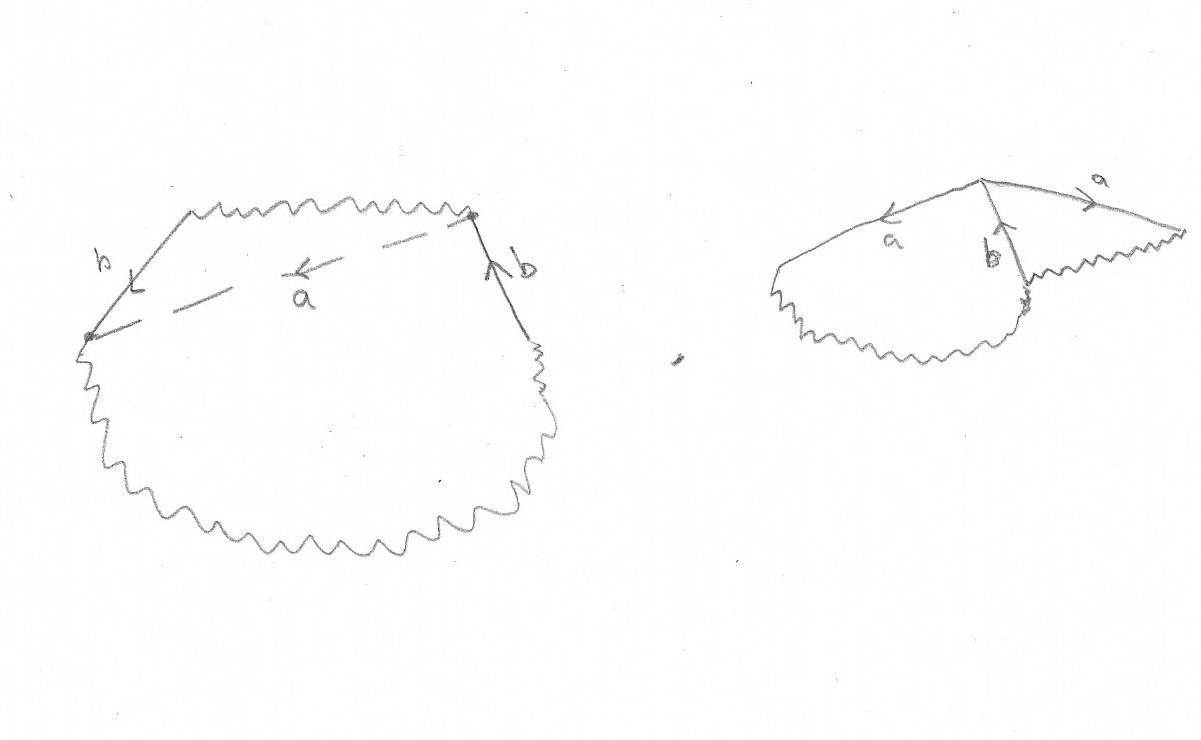
\includegraphics[width=10cm]{second.png}
     \caption{Making pairs of the second kind adjacent.}
     \label{fig:second-adjacent}
   \end{figure}

   If no pairs of the first kind are present at this stage, our
   polygon is of the form $a_1a_1a_2a_2 \dots a_na_n$: a connected sum
   of $n$ projective planes and we are done. We continue with the
   assumption that a pair of the first kind yet exists.

   We claim that a pair of the first kind must be separated by an edge
   of another pair of the first kind. To the
   contrary, consider the figure \ref{fig:first-contradiction}, where
   $A$ and $B$ respectively represent a sequences of pairs of the
   second kind (there are no pairs of the first kind other than $c$
   and $c^{-1}$ in the figure). Now by the step we have just
   completed, all pairs of the second kind are adjacent to one
   another. This means that each edge in $A$ has it's corresponding
   edge in $A$ and the same is true for $B$. But this means that
   the vertex at the origin and end of $c$ can't be identified with
   one another (the edges connecting to either end can never match),
   which means that we have at least 2 distinct equivalence classes of
   vertices, a contradiction of our previous step.

   \begin{figure}[htbp]
     \centering
     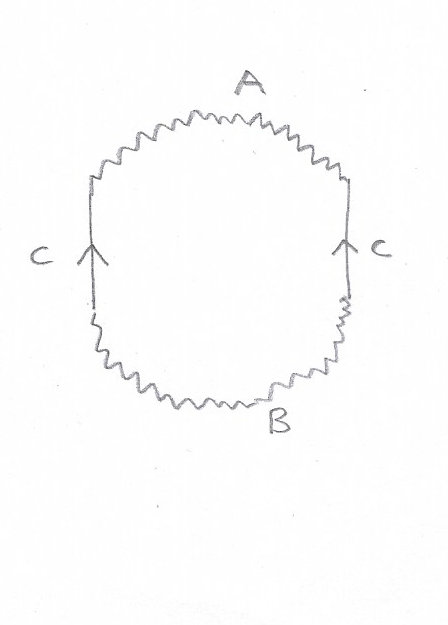
\includegraphics[width=8cm]{contr.png}
     \caption{A pair of the first kind separated on either side only
       by pairs of the second kind.}
     \label{fig:first-contradiction}
   \end{figure}

   Thus we assume that each pair of the first kind alternates with
   another pair of the first kind. The transformation pictured in
   figure \ref{fig:last} shows us how we can make these four edges
   adjacent. Now we can repeat this such that edges of the first kind
   always occur in fours. If no pairs of the second kind remain, we
   clearly have a connected sum of tori.

   On the other hand, if pairs of the second kind do remain, two
   alternating pairs of the second kind must be adjacent to such a
   pair. But lemma \ref{lem:connected} shows us that such an
   arrangement is equivalent to the connected sum of three projective
   planes; thus the whole polygon reduces to the connected sum of
   projective planes.

   \begin{figure}[htbp]
     \centering
     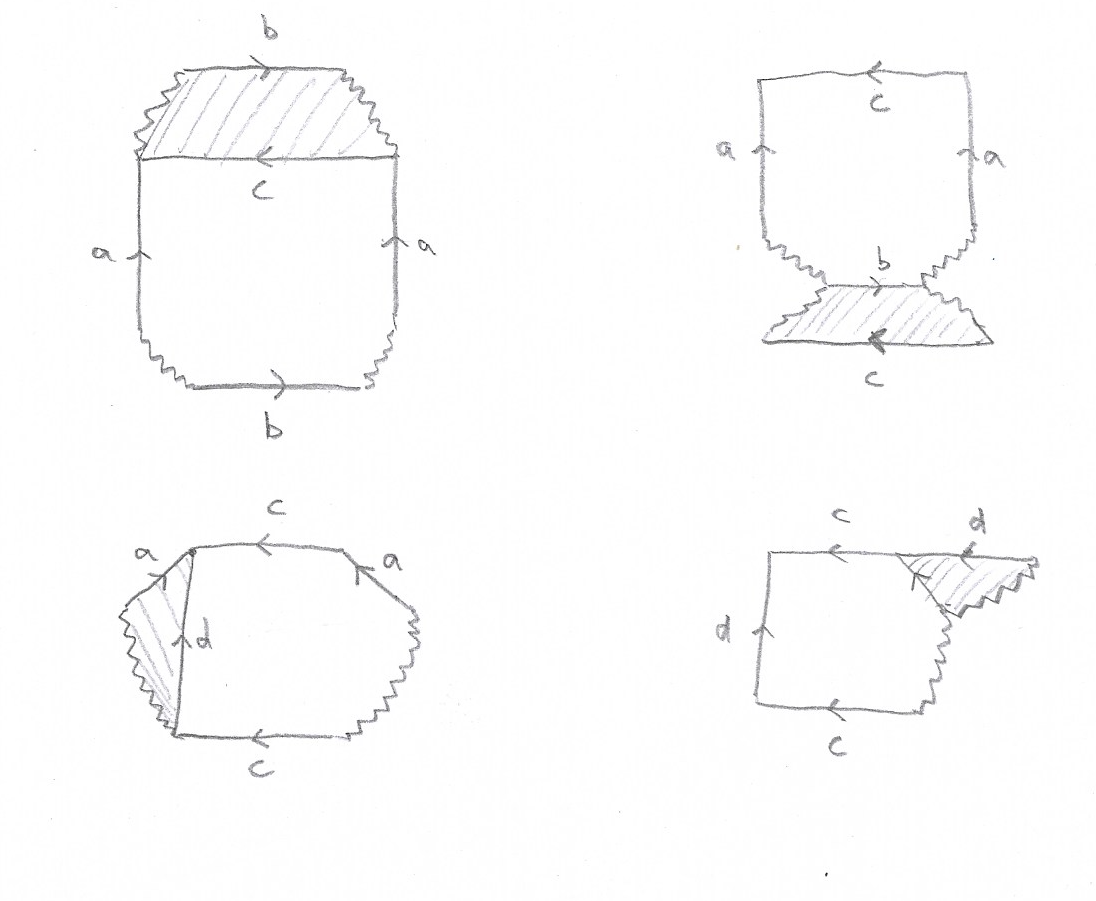
\includegraphics[width=8cm]{las.png}
     \caption{A pair of the first kind separated on either side only
       by pairs of the second kind.}
     \label{fig:last}          
   \end{figure}
 \end{proof}

 Thus we have classified an arbitrary compact connected surface without a boundary by triangulating it and forming a polygon from the triangulation which we manipulate into a canonical form. Our theorem can be extended without much difficulty to show that the compact surfaces with boundaries can be similarly classified into spheres or connected sums of projective planes and tori, however for each boundary present, we cut out a disc from the canonical surface. We have already seen this in the case of the M\"obius strip which is simply a projective plane with a disc cut out.



%%% Local Variables:
%%% mode: latex
%%% TeX-master: "main"
%%% End:
